\setcounter{topnumber}{5}
\setcounter{bottomnumber}{5}
\setcounter{totalnumber}{5}

\chapter{Procedimentos e resultados}

\section{Tarefa I}
\subsection{Procedimento}
\begin{description}
	\item[a)]Monte o circuito com a carga RL (1 K$\Omega$ em serie com um trimpot de 22K$\Omega$), sem o capacitor C e também sem o ramo contendo o diodo Zener.
	\item[b)] Imprima a forma de onda da tensão Vs do circuito, com o trimpot na posição de curto circuito.
	\item[c)] Compare a amplitude do valor da tensão obtida com o valor esperado.
	\item[d)] Comente ainda qual seria a amplitude do valor da tensão Vs , se utilizarmos o pino (3) ao invés do pino (2) do transformador?.
\end{description}
\subsection{Resultado}
\begin{description}
	\item[a)]Usando quatro diodos em configuração de ponte, a carga RL foi conectada em série nessa primeira parte, afim de analisar o comportamento da saída de onda.\\
	\centerline{\begin{minipage}[c]{\textwidth}
			\centering
			\noindent
			\captionof{figure}{Circuito retificador de onda completa}
			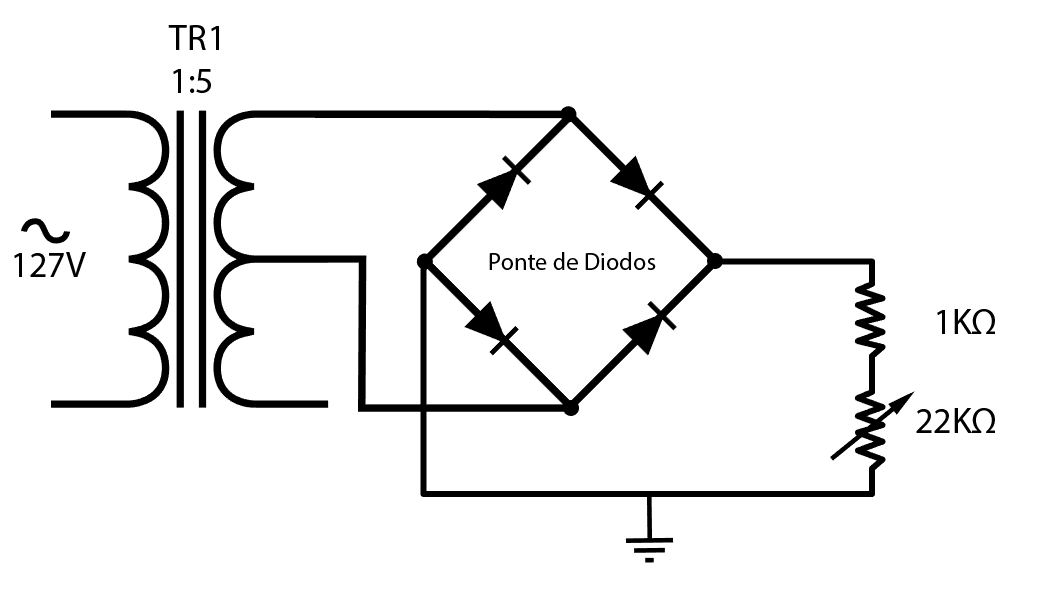
\includegraphics[width=0.5\textwidth]{Imagens/R1P1Im1.png}
			\label{Imagem1-birimba}
	\end{minipage}}
	\item[b)] A forma de onda, como mostrado na figura[numero da figura] é de um sinal retificado de onda completa, com tensão pico de 10,6V e tensão eficaz de 6.95V RMS.\\
	
	\centerline{\begin{minipage}[c]{\textwidth}
			\centering
			\noindent
			\captionof{figure}{Forma de onda}
			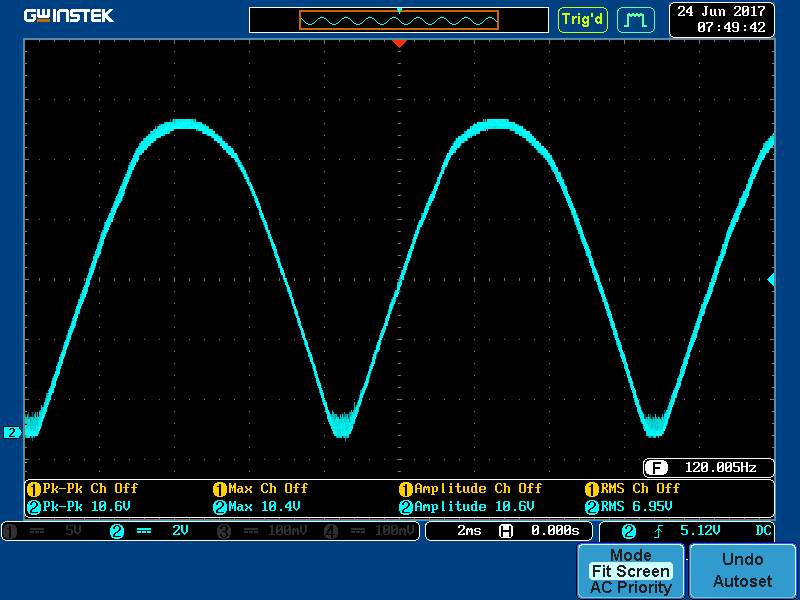
\includegraphics[width=0.5\textwidth]{Imagens/R1P2Im1.png}
			\legend{Fonte: \cite{Osciloscopio}}
			\label{imagem2 - birimba}
	\end{minipage}}
	
	\item[c)] Neste experimento foi usado um transformador abaixador de 1:5 com derivação central no secundário, e a ponte de diodos foi conectada aos pinos 1 e 2, fazendo com que a queda de tensão caia pela metade. Como a fonte de alimentação é de 127v RMS, a tensão entre os pino 1 e 3 do secundário do transformador deveria ser de aproximadamente 25,4V, e a tensão entre os pinos 1 e 2 do secundário deveria ser a metade disso, ou seja 12,7V.
	Com o circuito montado com a ponte de diodos, a carga de 1K$\Omega$  e o trimpot de 22K$\Omega$ a tensão de pico na carga deveria ser de 12V.
	As perdas dos valores ideais a serem obtidos e os valores que realmente foram apresentados durante o experimento em laboratório são normais, e são causadas por inúmeros fatores que vão desde a fabricação dos componentes como a montagem do circuito.\\
	
	\centerline{\begin{minipage}[c]{\textwidth}
			\centering
			\noindent
			\captionof{figure}{Dados referentes a onda}
			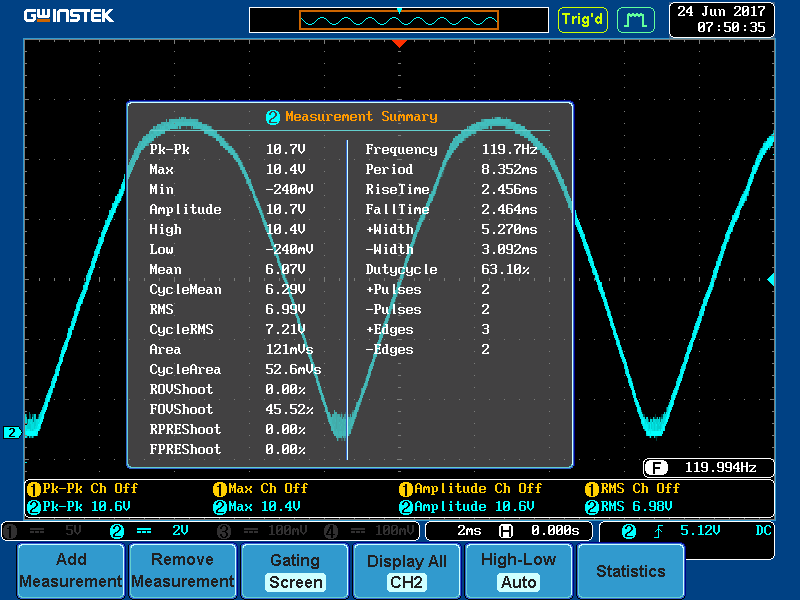
\includegraphics[width=0.5\textwidth]{Imagens/R1P3Im1.png}
			\legend{Fonte: \cite{Osciloscopio}}
			\label{}
	\end{minipage}}

	\item[d)]Como dito antes, neste experimento foi usado um transformador abaixador de 1:5 com derivação central no secundário, a diferença de potencial, caso os pinos 1 e 3 do secundário fossem utilizados seria exatamente o dobro das medidas obtidas nesse experimento.
\end{description}

\section{Tarefa II}
\subsection{Procedimentos}
Ligue o capacitor eletrol\'itico de $100 \mu$F em paralelo com a carga $R_L$ no circuito anterior. Imprima a forma de onda da tens\~ao $V_s$, com o trimpot na posiç\~ao de curto. Compare-a com o sinal obtido anteriormente.

Qual é a funç\~ao do capacitor? Comente os resultados esperados se variarmos o valor da resist\^encia de carga e da capacit\^ancia.
\subsection{Resultados}
Com a liga\c{c}\~ao do capacitor eletrol\'itico, nesse experimento usamos um de $470 \mu$F, em paralelo com a carga $R_L$, obtemos a seguinte forma de onda, representada na figura 1 b, em compara\c{c}\~ao ao resultado anterior, figura 1 a, temos que com o capacitor, o tamanho da onda diminuiu muito, tendo uma varia\c{c}\~ao muito menor do que a anterior, tendo um valor muito mais constante. Tendo assim como fun\c{c}\~ao do capacitor nesse circuito, como um filtro, onde com a filtragem a ondula\c{c}\~ao fica menor da onda, se comparando a tens\~ao cont\'inua. 

\centerline{{\begin{minipage}[b]{0.5\textwidth}
			\centering
			\captionof{figure}{Sem capacitor}
			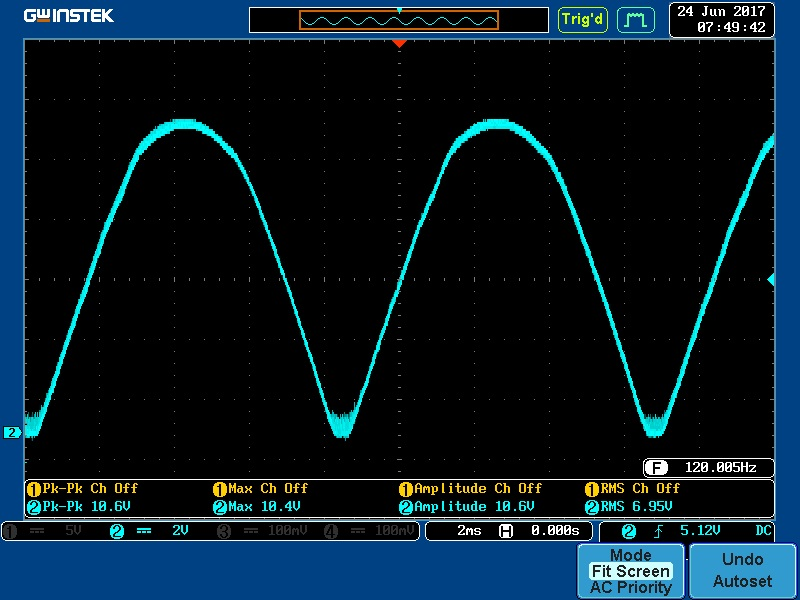
\includegraphics[width=\textwidth]{Imagens/sem_capacitor.jpg}
			\legend{Fonte:\cite{Osciloscopio}}
		\end{minipage}
		\hfill
		\begin{minipage}[b]{0.5\textwidth}
			\centering
			\captionof{figure}{Com Capacitor}
			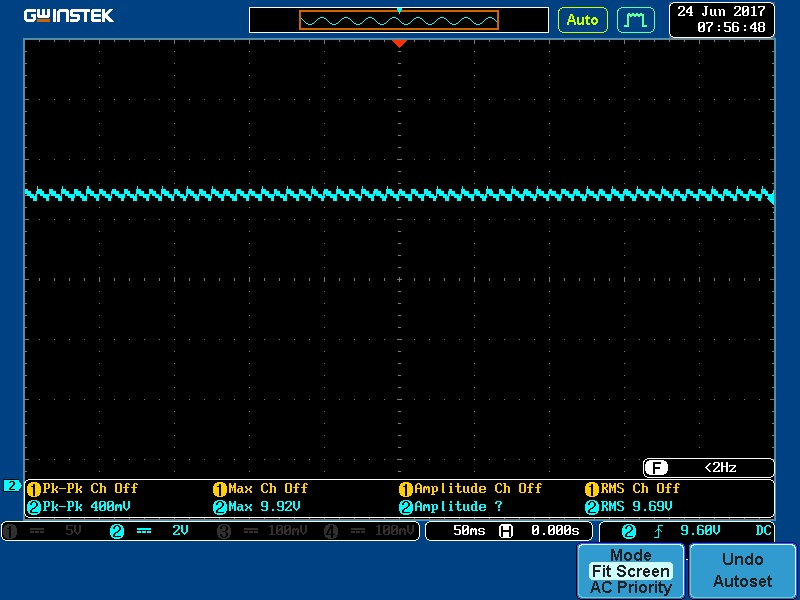
\includegraphics[width=\textwidth]{Imagens/capacitor_filtro.jpg}		
			\legend{Fonte:\cite{Osciloscopio}}
\end{minipage}}}

\centerline{Forma de onda da tensão $V_s$}

Quando variamos a resist\^encia, variamos a tens\~ao m\'axima de sa\'ida, sendo proporcional, ou seja, com o aumento na resist\^encia, a tens\~ao ser\'a maior e com o uma diminui\c{c}\~ao teremos uma tens\~ao menor. Em rela\c{c}\~ao a varia\c{c}\~ao na capacit\^ancia, \'e proporcionalmente a filtragem, ou seja, quanto maior a capacit\^ancia menor ser\'a a varia\c{c}\~ao da onda, tendo uma menor ondula\c{c}\~ao e quando menor a capacit\^ancia maior ser\'a a varia\c{c}\~ao da onda.

\section{Tarefa III}
\subsection{Procedimentos}
\begin{description}
	\item[a)] Ligue agora o diodo Zener (1N4738 ou um similar de 2,1V, 3,2V 5,1V) em série com Rl.
	\item[b)] Verifique se Rl = 1 K$\Omega$ é suficiente para limitar a corrente no diodo para evitar superaquecimento e ligue-o em série com o diodo.
	\item[c)] Observe com o osciloscópio a forma de onda de Vz e compare-a com as observadas nos itens anteriores. Comente os resultados obtidos.
\end{description}

\subsection{Resultados}
\begin{description}
	\item[a)] Com a adição dos últimos componentes, o circuito agora está completo.\\
	
	\centerline{\begin{minipage}[c]{\textwidth}
			\centering
			\noindent
			\captionof{figure}{Representaçao do circuito montado}
			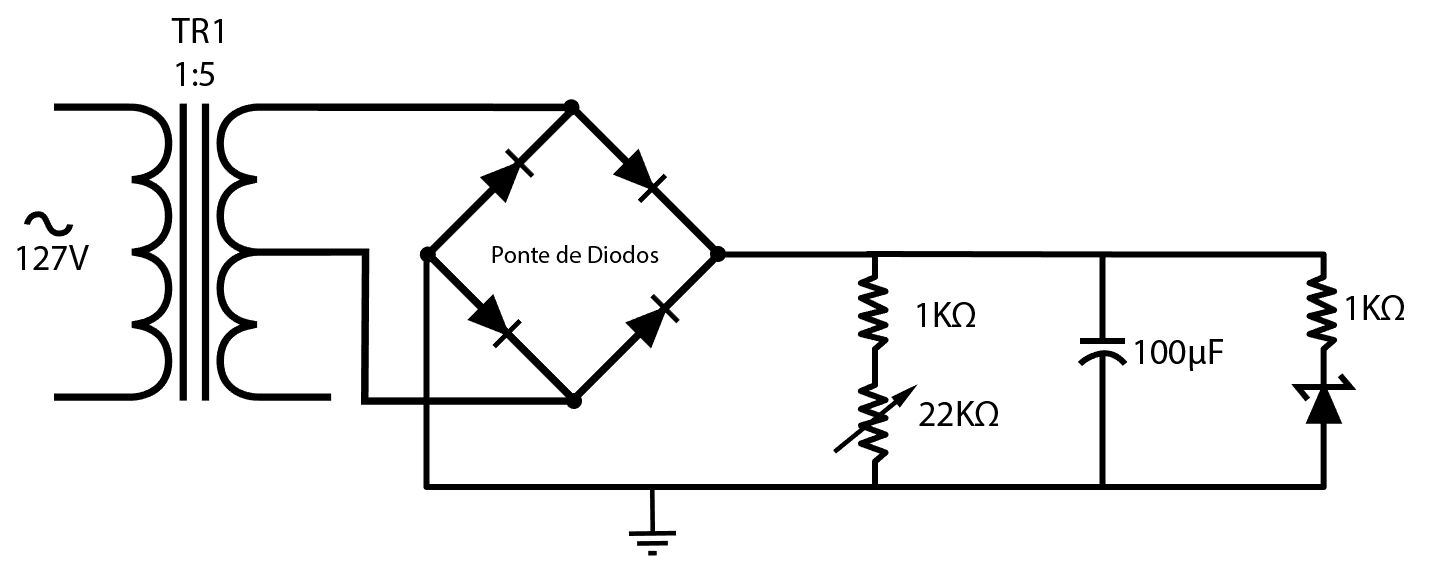
\includegraphics[width=0.5\textwidth]{Imagens/R3P1Im1.png}
			\label{}
	\end{minipage}}
	
	\item[b)] Antes de conectar Diodo Zener ao circuito, foi feito um teste rápido afim de verificar a temperatura do componente caso ele fosse adicionado ao circuito. O resultado foi satisfatório, não apresentando superaquecimento, caso contrário a resistência de 1K$\Omega$ seria substituída por outra de valor maior.
	\item[c)] Como podemos ver no gráficos abaixo da saída de tensão, o diodo zener teve a função de estabilizar a saída da onda do capacitor, visto que esta oscilava bastante e não seria um sinal satisfatório para o uso prático. O diodo zener serviu como um filtro, e deixou o sinal o sinal com o mínimo de trepidações. É claro que o resultado não é exatamente perfeito como os obtidos em simuladores, mas a trepidação existente é pequena a um nível que pode ser ignorada.\\

	\centerline{\begin{minipage}[c]{\textwidth}
			\centering
			\noindent
			\captionof{figure}{Forma de onda}
			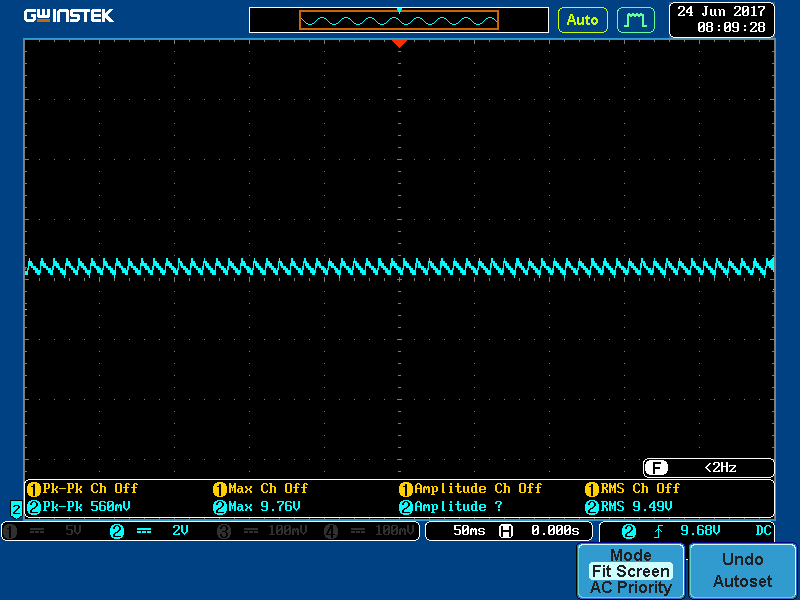
\includegraphics[width=0.5\textwidth]{Imagens/R3P3Im1.png}
			\legend{Fonte: \cite{Osciloscopio}}
			\label{}
	\end{minipage}}

	\centerline{\begin{minipage}[c]{\textwidth}
			\centering
			\noindent
			\captionof{figure}{Dados obtidos}
			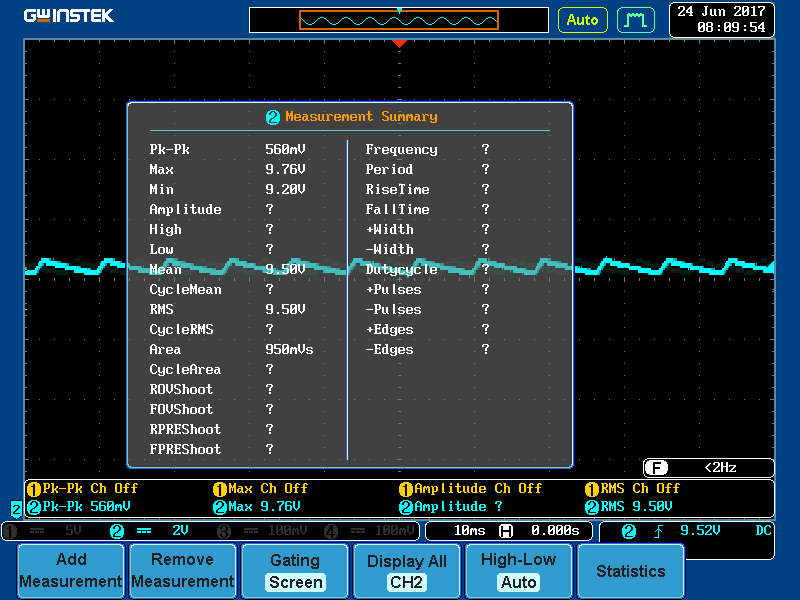
\includegraphics[width=0.5\textwidth]{Imagens/R3P3Im2.png}
			\legend{Fonte: \cite{Osciloscopio}}
			\label{}
	\end{minipage}}

\end{description}

\section{Tarefa IV}
\subsection{Procedimento}
Explique o funcionamento do diodo Zener?
\subsection{Resultado}
Alguns diodos possuem a característica especial de operação na região de ruptura, onde grandes variações de corrente resultam em pequenas variações de tensão, a esse dispositivo chamamos Diodo Zener. 
É importante ressaltar que quando polarizado diretamente, ele atua como um diodo comum, conduzindo a partir de 0,7 V e ao ser inversamente polarizado, atua como zener.
Suas principais características elétricas são:
\begin{itemize}
	\item A tensão Zener é especificada pelo fabricante e geralmente abreviada à VZ;
	\item A corrente mínima de operação do Zener na região de ruptura é IKZ;
	\item A corrente máxima para o trabalho do Zener é IZM e se ultrapassado tal valor, o diodo será destruído;
	\item A PW é a potência máxima dissipada pelo Zener (No diodo usado no experimento, pode ser dissipado até 1W);
	\item A RZ é a resistência do Zener;
	\item VZ é a tolerância de tensão do diodo Zener.
\end{itemize}

\noindent A curva característica do zener é mostrada na figura abaixo:

\centerline{\begin{minipage}[c]{\textwidth}
		\centering
		\noindent
		\captionof{figure}{Curva característica do diodo Zener}
		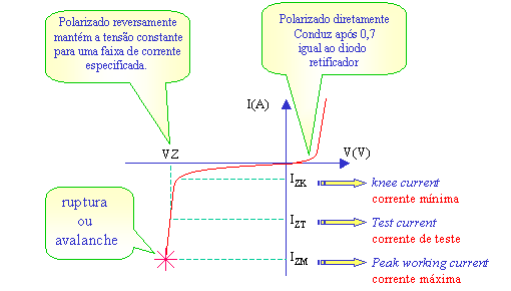
\includegraphics[width=0.5\textwidth]{Imagens/R4PUIm1.png}
		\legend{Fonte: \cite{R4PUIm1}}
		\label{}
\end{minipage}}

\noindent Abaixo a simbologia usual do diodo Zener:

\centerline{\begin{minipage}[c]{\textwidth}
		\centering
		\noindent
		\captionof{figure}{Simbologia do Zener}
		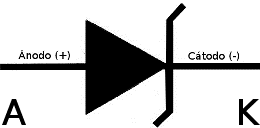
\includegraphics[width=0.5\textwidth]{Imagens/R4PUIm2.png}
		\legend{Fonte: \cite{R4PUIm2}}
		\label{}
\end{minipage}}